% mensaje del parafo:
% utilidad de la seleccion de caracteristicas en datos sanitarios
Applying Feature Selection techniques to medical data such as clinical, genomic, proteomic or metabolomic information could solve two important medical problems. One problem is related to the task of finding which are the relevant variables involved in a disease, response to treatment, survival time, relapse probability, etc. It could lead to understand better the disease mechanisms, evaluate the factors that are involved or even propose new hypotheses about factors that have not been taken into account until this moment. The second problem is to perform variable reduction and learn a predictive model with the best possible performance to cost ratio by using the minimum set of diagnostic variables. This estimator could then be used as an aid in clinical decisions or as an indicator for research. In this case, the focus can be moved from the relevancy of the reduced variable subset to the final performance of the model. 
\\

% mensaje del parafo:
% complejidad de los datos sanitarios (pocas observaciones, muchas variables)
Despite the considerable efforts made in capturing health data, the common situation is still having much more variables than observations (individuals). While the number of observations is usually around hundreds or thousands, the number of variables could reach millions. This is an unfavourable condition for any Machine Learning algorithm (Bellman's curse of dimensionality \cite{Bellman2015AdaptiveTour}). 
\\

% mensaje del parafo:
% aproximacion Ensemble para resolverlo pero nueva limitacion con las variables rivales
Ensemble Feature Selection has been receiving an increasing attention during the last decade \cite{Bolon-Canedo2019EnsemblesTrends} \cite{Pes2020EnsembleDomains} \cite{Abeel2009RobustMethods} \cite{BenBrahim2017EnsembleStudy} and consists in combining the output of several inducers applied on distinct subset of a database. It results in an improvement of the selection stability and robustness to the lack of observations. Nevertheless, more work is required especially with relevant but redundant variables which tend not to be selected. 
\\

Indeed, redundant variables are competing for the vote inside the ensemble approach reducing their possibilities to get selected.
\\

% mensaje del parafo:
% objetivo del estudio: identificar las variables rivales para agruparlas y mejorar la calidad de la lista de relevantes proporcionado por la seleccion Ensemble
% TODO
In the rest of the document, redundant variable are also called rival variables. We aim to identify rival variants among the feature set items, which we group in order to propose an improved list of relevant features that contribute to a better prediction of disease cases. There are no direct biological insights to be found in this project, nor biomarkers to be discovered, although further research on the shared list might lead to this outcome. Also, we study the behaviour of Ensemble Feature Selection with redundant variables, interaction of which is commonly unknown and intricate to decipher \cite{Saeys2007ABioinformatics}.
\\

% mensaje de la seccion:
% presentar el algoritmo Ensemble para poder explicar correctamente el swapper en la parte 2.x. algoritmo swapper (o como se llame)
The workflow of the Ensemble Feature Selection we used internally to obtain the starting data of this work is described in Figure \ref{fig:Ensemble-diagram}. Its understanding is essential for building our workflow since it relies on an \emph{Ensemble} generated object.
\\

\begin{figure}[!htpb]
    \centering
    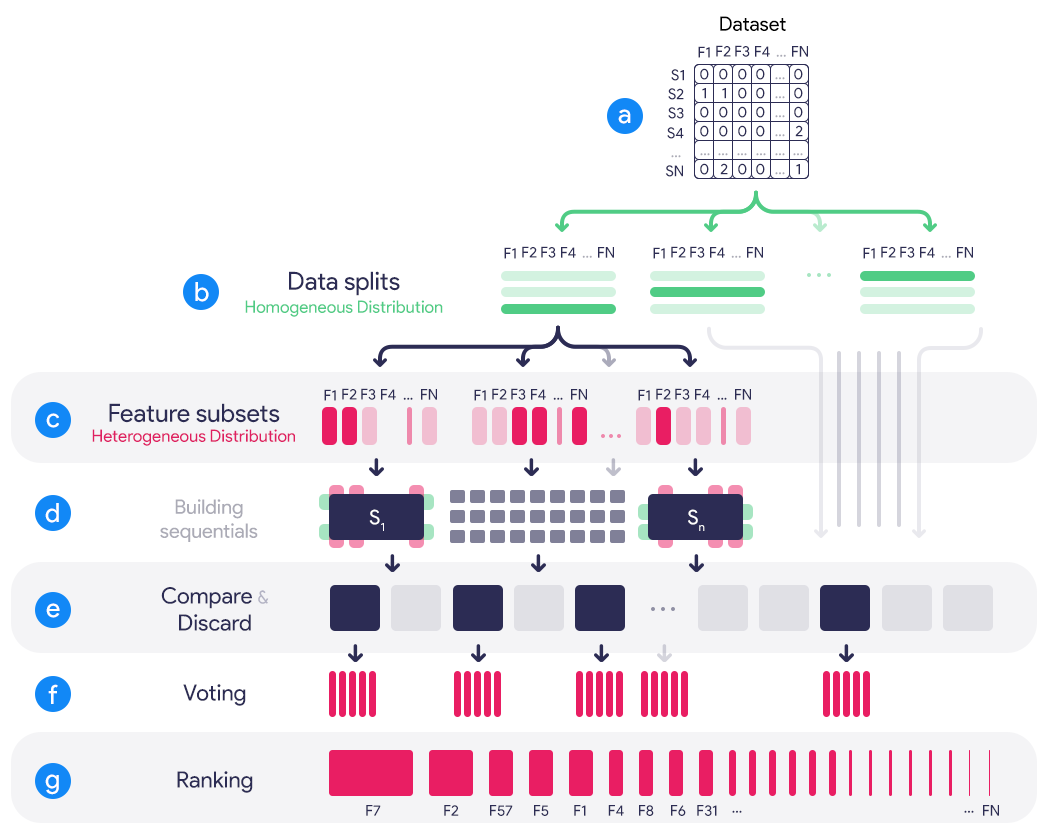
\includegraphics[width=\linewidth]{Minor Thesis/figures/diagrams/Ensemble.png}
    \caption{Ensemble workflow. (a) Dataset in matrix format. (b) Resampling data \emph{without replacement}. (c) Apply several feature selectors to each split, then evaluate their performance iteratively to achieve the best predictive variable subset. Each run delivers a \emph{Sequential}. (d) Discard Sequentials which have poor predictive power. (e) Aggregate Sequentials results: Each feature appearance in a Sequential result adds a vote to the feature. (f) Return the full list of ranked features, discarding those which have not obtained enough votes over the threshold.}
    \label{fig:Ensemble-diagram}
\end{figure}

Ensemble approach attempts to combine different opinions from a group of estimators working on several splits of a dataset. For each set of data, a subset of features that best predicts the task is computed, hence multiple results consensus delivers a multi-perspective observation of the problem. 
\\

In our particular case, an \epmh{Ensemble} assigns a vote to a variable each time this variable belongs to a valid Sequential. A Sequential\footnote{Several approaches are available, but this project focuses on \href{http://rasbt.github.io/mlxtend/user_guide/feature_selection/SequentialFeatureSelector/}{forward/backward} Sequentials since they use an \emph{overall approach} when considering data.} is a weak feature selector. It uses a greedy approach and, although their computation tends to be heavy, they tend to be powerful and complete. Sequential validation is based on a minimum threshold accuracy, termination and error-free behaviour.
\\

% OK
When an Ensemble method attempts to assign votes to all variables, those features which hold a significant similarity might alternately receive the votes. E.g. assuming X and Y obtain 5 and 10 votes respectively and they hold a similarity of 95\%, their prediction might have been the same since they are highly similar at the eyes of the classifier. The total maximum of votes (15) has been split in two variables, and both have lost positions in the ranking. We name this phenomenon \emph{rivalry}.

Either highly redundant features (due to quasi-constant values, etc.) or features holding a strong rivalry, hamper Ensemble's aim to identify every relevant variable, and, ultimately, accurately rank variants.
\\

In this project we introduce an approach which performs an iterative swap between each of the variants in a feature set (already calculated in an individual Sequential) and the features picked by the full Ensemble --as a result of a consensus function and which are not contained yet in the original feature set-- in order to perform a retraining of the Sequentials and further compare the prediction results.
\\

This new approach will be added and assessed against other ways of clustering votes and correcting ranks.
\\

In our definition of rivalry, two variables compete against each other with regard to a subset of variables if swapping them does not change the prediction.
More precisely, if the original prediction (A) and the set-swapped prediction (B), are similar more than a custom threshold (overlap(A, B) >= threshold), we consider the pair of features swapped are highly linked.
\\

Therefore, assessing one-to-one prediction similarity and investigating paired correlation allows us to re-rank the original Ensemble output, helping us to tackle the vote rivalry problem. This assists the Maximum Relevance Minimum Redundancy (MRMR) \cite{Auffarth2010ComparisonImages}\cite{Peng2005FeatureMin-Redundancy} approach used in problems which face up dimensionality issues by reducing redundancy.